%%%%%%%%%%%%%%%%%%%%%%%%%%%%%%%%%%%%%%%%%%%%%%%%%%%%%%%%%%%%%%%%%%%
%%% Documento LaTeX                                             %%%
%%%%%%%%%%%%%%%%%%%%%%%%%%%%%%%%%%%%%%%%%%%%%%%%%%%%%%%%%%%%%%%%%%%
% Título:   Apéndice A
% Autor:    Ignacio Moreno Doblas
% Fecha:    2014-02-01
% Versión:  0.5.0
%%%%%%%%%%%%%%%%%%%%%%%%%%%%%%%%%%%%%%%%%%%%%%%%%%%%%%%%%%%%%%%%%%%%

\pagestyle{fancy}
\fancyhead[LE,RO]{\thepage}
\fancyhead[RE]{Apéndice} %
\fancyhead[LO]{\nouppercase{\rightmark}}
%\fancyhead[RE]{Parte \thepart \rightmark} %

\chapterbegin{Resistencias programables de pull-up y pull-down}
\label{chp:resistencias}
\minitoc

\section{Introducción}

En general las resistencias de pull-up y pull-down son resistencias que se ponen en
las entradas para fijar la tensión que de otra forma quedaría indeterminada, al estar
en situación de circuito abierto o alta impedancia. El ejemplo típico donde se usa es
en un pulsador. Eléctricamente un pulsador no es más que un interruptor que deja pasar
la corriente cuando está pulsado y se queda en circuito abierto en su posición de reposo
(sin pulsar). De los dos contactos que tiene, uno se conecta a masa y el otro al pin de
entrada de la Raspberry. Así que cuando lo pulsamos hacemos un corto que llevaría los cero
voltios de la masa al pin de entrada (enviamos un cero lógico), pero cuando está sin pulsar
no enviamos nada al pin, éste se queda en lo que se denomina alta impedancia.

Todos los pines del GPIO en la Raspberry se pueden configurar por software para que
se comporten como queramos: o bien sin resistencia, o con una resistencia a Vcc (pull-up) o
con una resistencia a masa (pull-down). Este tipo de resistencias son débiles (weak) debido
a que están dentro de la pastilla (SoC) y se implementan con transistores. Se puede
anular el efecto de estas resistencias poniendo resistencias externas.

\section{Pulsadores en la placa auxiliar}

En la placa auxiliar tenemos dos pulsadores conectados a GPIO 2 y GPIO 3. No es casualidad
que estén conectados concretamente a esos dos pines. Son los únicos pines que tienen
resistencias externas de pull-up, concretamente de 1K8, que anulan cualquier configuración
interna que pongamos. La razón es porque las resistencias internas son débiles, tienen un
valor aproximado de unos 50K. Cuando hay dos resistencias en paralelo como es el caso,
la de menor valor anula el efecto de la de mayor valor.

Por tanto si configuramos GPIO 2 ó GPIO 3 como entradas, independientemente del valor
que configuremos por software, se comportarán siempre como si sólo tuviesen una
resistencia de pull-up.

El propósito de este apéndice es aprender a cambiar la configuración de los pull-ups/pull-downs
en caso de usar otras placas auxiliares distintas. En la nuestra las únicas entradas (pulsadores)
que hay están resueltas con las resistencias antes comentadas que tiene la Raspberry sólo en
esos dos pines.

\section{Ejemplo de aplicación}

El montaje que proponemos es con uno de los pines de la fila superior, en concreto el
pin GPIO 18 que hay a la derecha de los pines del puerto serie. En estos ejemplos
no vamos a requerir la placa auxiliar, de esta forma
dejamos libres los pines Vcc (3.3V), ya que necesitaremos uno para el último ejemplo. 

\subsection{Pulsador a masa sin cambiar configuración}

En este primer ejemplo vamos a tratar de encender el LED interno de la Raspberry llamado
ACT (OK) mediante un pulsador externo. El primer montaje sería el de
la figura.

El esquema sería el de la figura \ref{fig:circuito1}.

\begin{figure}[h]
  \centering
    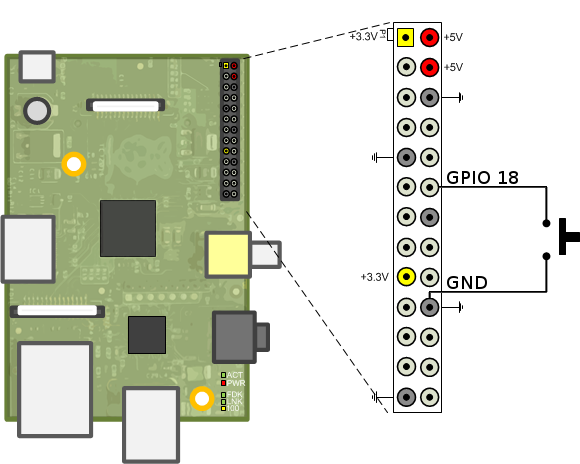
\includegraphics[width=14cm]{graphs/circuito1.png}
  \caption{Pulsador a masa}
  \label{fig:circuito1}
\end{figure}

Ahora escribimos el código. Como el pin GPIO que controla dicho LED es distinto en los
modelos normales que en los A+/B+, enviamos la señal a ambos pines. En el modelo normal
sería GPIO 16 y en el plus, el GPIO 47.

\begin{lstlisting}[caption={apend1.s},label={lst:codigoApendice_1}]
        .include  "inter.inc"
.text
        ldr     r0, =GPBASE
/* guia bits           xx999888777666555444333222111000*/
        mov     r1, #0b00000000000001000000000000000000
        str     r1, [r0, #GPFSEL1]
/* guia bits           xx999888777666555444333222111000*/
        mov     r1, #0b00000000001000000000000000000000
        str     r1, [r0, #GPFSEL4]
/* guia bits           10987654321098765432109876543210*/
        mov     r2, #0b00000000000000010000000000000000
/* guia bits           32109876543210987654321098765432*/
        mov     r3, #0b00000000000000001000000000000000
bucle:  str     r2, [r0, #GPCLR0]   @ apago GPIO 16
        str     r3, [r0, #GPCLR1]   @ apago GPIO 47
        ldr     r1, [r0, #GPLEV0]
/* guia bits           10987654321098765432109876543210*/
        tst     r1, #0b00000000000001000000000000000100
        streq   r2, [r0, #GPSET0]   @ enciendo GPIO 16
        streq   r3, [r0, #GPSET1]   @ enciendo GPIO 47
        b       bucle
\end{lstlisting}

Probamos el código y comprobamos que al pulsar el botón izquierdo no pasa nada,
el LED está siempre encendido.

Esto se debe a que por defecto el pin GPIO 18 está configurando con una resistencia de
pull-down y nosotros necesitamos una de pull-up, de lo contrario siempre leeremos un cero
por dicho pin. Los valores por defecto (tras el reset) se pueden consultar en la página
103 del datasheet, aunque la mayor parte de los pines disponibles por el puerto estan
a pull-down.

Para solventar ésto hay tres opciones: o conectar el otro terminal del interruptor a Vcc en
lugar de a GND, o configurar el pin para cambiarlo de pull-down a pull-up, o conectar una
resistencia externa a Vcc que anule el pull-down interno. Nosotros vamos a explorar las dos
primeras opciones.

\subsection{Pulsador a masa cambiando configuración}

En este ejemplo vamos a configurar GPIO 18 a pull-up de acuerdo a la siguiente
figura \ref{fig:pullup}.

\begin{figure}[h]
  \centering
    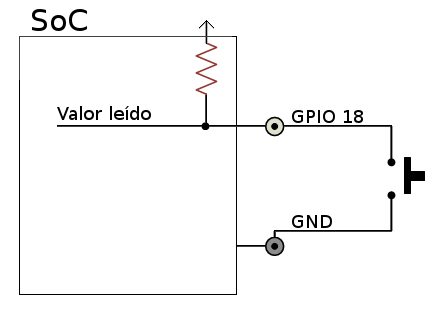
\includegraphics[width=14cm]{graphs/pullup.png}
  \caption{Resistencia interna de pull-up}
  \label{fig:pullup}
\end{figure}

Para configurar un pin determinado en pull-up/pull-down/desconectado seguimos los
siguientes pasos.

\begin{enumerate}
  \item Escribir en {\tt GPPUD} el tipo de resistencia que queremos. Un 0 sería
si no queremos resistencia, un 1 si es de pull-down ó un 2 si lo que queremos es un
pull-ups.
  \item Esperar 150 ciclos. Esto provee el tiempo requerido de {\tt set-up} para controlar la señal.
  \item Escribir en {\tt GPPUDCLK0/1} un 1 en la posición de los pines que queramos modificar,
mientras que los que estén a 0 mantendrán su antiguo estado.
  \item Esperar otros 150 ciclos. Con esto le damos tiempo de {\tt hold} suficiente a la señal.
  \item Poner GPPUD en su estado de reposo, que sería a valor 0 (desactivado).
  \item Escribir un 0 en {\tt GPPUDCLK0/1}.
\end{enumerate}

Una de las cosas que tenemos que hacer es esperar 150 ciclos (como mínimo). Como
sabemos que un salto condicional tarda al menos dos ciclos en ejecutarse, nuestra rutina
de retardo sería la siguiente.

\begin{lstlisting}
wait:   mov     r1, #50
wait1:  subs    r1, #1
        bne     wait1
        bx      lr
\end{lstlisting}

Y el código que hace todo lo anterior, para poner a pull-up el GPIO 18 (donde hemos puesto
el pulsador) es el siguiente.

\begin{lstlisting}
        str     r1, [r0, #GPPUD]
        bl      wait
/* guia bits           10987654321098765432109876543210*/
        mov     r1, #0b00000000000001000000000000000100
        str     r1, [r0, #GPPUDCLK0]
        bl      wait
        mov     r1, #0
        str     r1, [r0, #GPPUD]
        str     r1, [r0, #GPPUDCLK0]
\end{lstlisting}

El ejemplo completo quedaría así.

\begin{lstlisting}[caption={apend2.s},label={lst:codigoApendice_2}]
        .include  "inter.inc"
.text
        ldr     r0, =GPBASE
/* guia bits           xx999888777666555444333222111000*/
        mov     r1, #0b00000000000001000000000000000000
        str     r1, [r0, #GPFSEL1]
/* guia bits           xx999888777666555444333222111000*/
        mov     r1, #0b00000000001000000000000000000000
        str     r1, [r0, #GPFSEL4]
        mov     r1, #2
        str     r1, [r0, #GPPUD]
        bl      wait
/* guia bits           10987654321098765432109876543210*/
        mov     r1, #0b00000000000001000000000000000100
        str     r1, [r0, #GPPUDCLK0]
        bl      wait
        mov     r1, #0
        str     r1, [r0, #GPPUD]
        str     r1, [r0, #GPPUDCLK0]
/* guia bits           10987654321098765432109876543210*/
        mov     r2, #0b00000000000000010000000000000000
/* guia bits           32109876543210987654321098765432*/
        mov     r3, #0b00000000000000001000000000000000
bucle:  str     r2, [r0, #GPCLR0]   @ apago GPIO 16
        str     r3, [r0, #GPCLR1]   @ apago GPIO 47
        ldr     r1, [r0, #GPLEV0]
/* guia bits           10987654321098765432109876543210*/
        tst     r1, #0b00000000000001000000000000000100
        streq   r2, [r0, #GPSET0]   @ enciendo GPIO 16
        streq   r3, [r0, #GPSET1]   @ enciendo GPIO 47
        b       bucle

wait:   mov     r1, #50
wait1:  subs    r1, #1
        bne     wait1
        bx      lr
\end{lstlisting}

Comprobamos cómo ahora sí funciona, y mientras tenemos el botón presionado,
el LED se enciende, apagándose en cuanto lo soltamos.

\subsection{Pulsador a Vcc sin cambiar configuración}

Cambiamos es montaje, y en lugar de a GND conectamos el pulsador a Vcc según
la figura \ref{fig:circuito2}.

\begin{figure}[h]
  \centering
    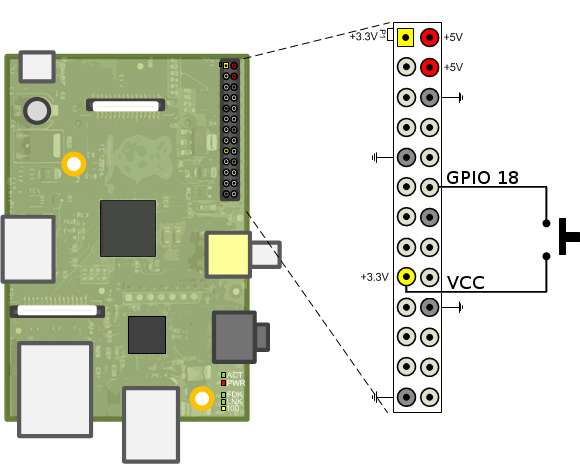
\includegraphics[width=14cm]{graphs/circuito2.png}
  \caption{Pulsador a Vcc}
  \label{fig:circuito2}
\end{figure}

De esta forma aprovechamos que ese pin en concreto está conectado a pull-down tras
el reset, por lo que no habría que cambiar la configuración del pin para obtener
lo que vemos en la figura \ref{fig:pulldown}.

Prácticamente tendríamos el mismo código que en {\tt apend1.s} no nos funcionaba,
la única diferencia es que cambiamos los {\tt streq} por {\tt strne}.

\begin{lstlisting}[caption={apend3.s},label={lst:codigoApendice_3}]
        .include  "inter.inc"
.text
        ldr     r0, =GPBASE
/* guia bits           xx999888777666555444333222111000*/
        mov     r1, #0b00000000000001000000000000000000
        str     r1, [r0, #GPFSEL1]
/* guia bits           xx999888777666555444333222111000*/
        mov     r1, #0b00000000001000000000000000000000
        str     r1, [r0, #GPFSEL4]
/* guia bits           10987654321098765432109876543210*/
        mov     r2, #0b00000000000000010000000000000000
/* guia bits           32109876543210987654321098765432*/
        mov     r3, #0b00000000000000001000000000000000
bucle:  str     r2, [r0, #GPCLR0]   @ apago GPIO 16
        str     r3, [r0, #GPCLR1]   @ apago GPIO 47
        ldr     r1, [r0, #GPLEV0]
/* guia bits           10987654321098765432109876543210*/
        tst     r1, #0b00000000000001000000000000000100
        strne   r2, [r0, #GPSET0]   @ enciendo GPIO 16
        strne   r3, [r0, #GPSET1]   @ enciendo GPIO 47
        b       bucle
\end{lstlisting}

\begin{figure}[h]
  \centering
    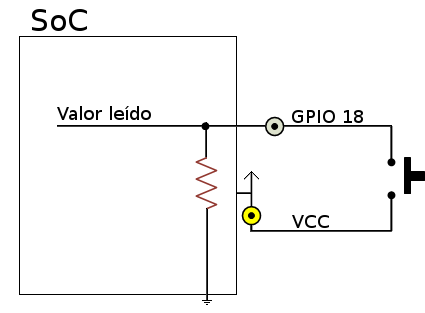
\includegraphics[width=14cm]{graphs/pulldown.png}
  \caption{Resistencia interna de pull-down}
  \label{fig:pulldown}
\end{figure}

\chapterend
